\documentclass{article}
\usepackage{graphicx}
\usepackage{a4wide}
\usepackage[colorlinks, linkcolor=black]{hyperref}
\usepackage{color}
\usepackage[T1]{fontenc}
\begin{document}


\begin{figure}[th]
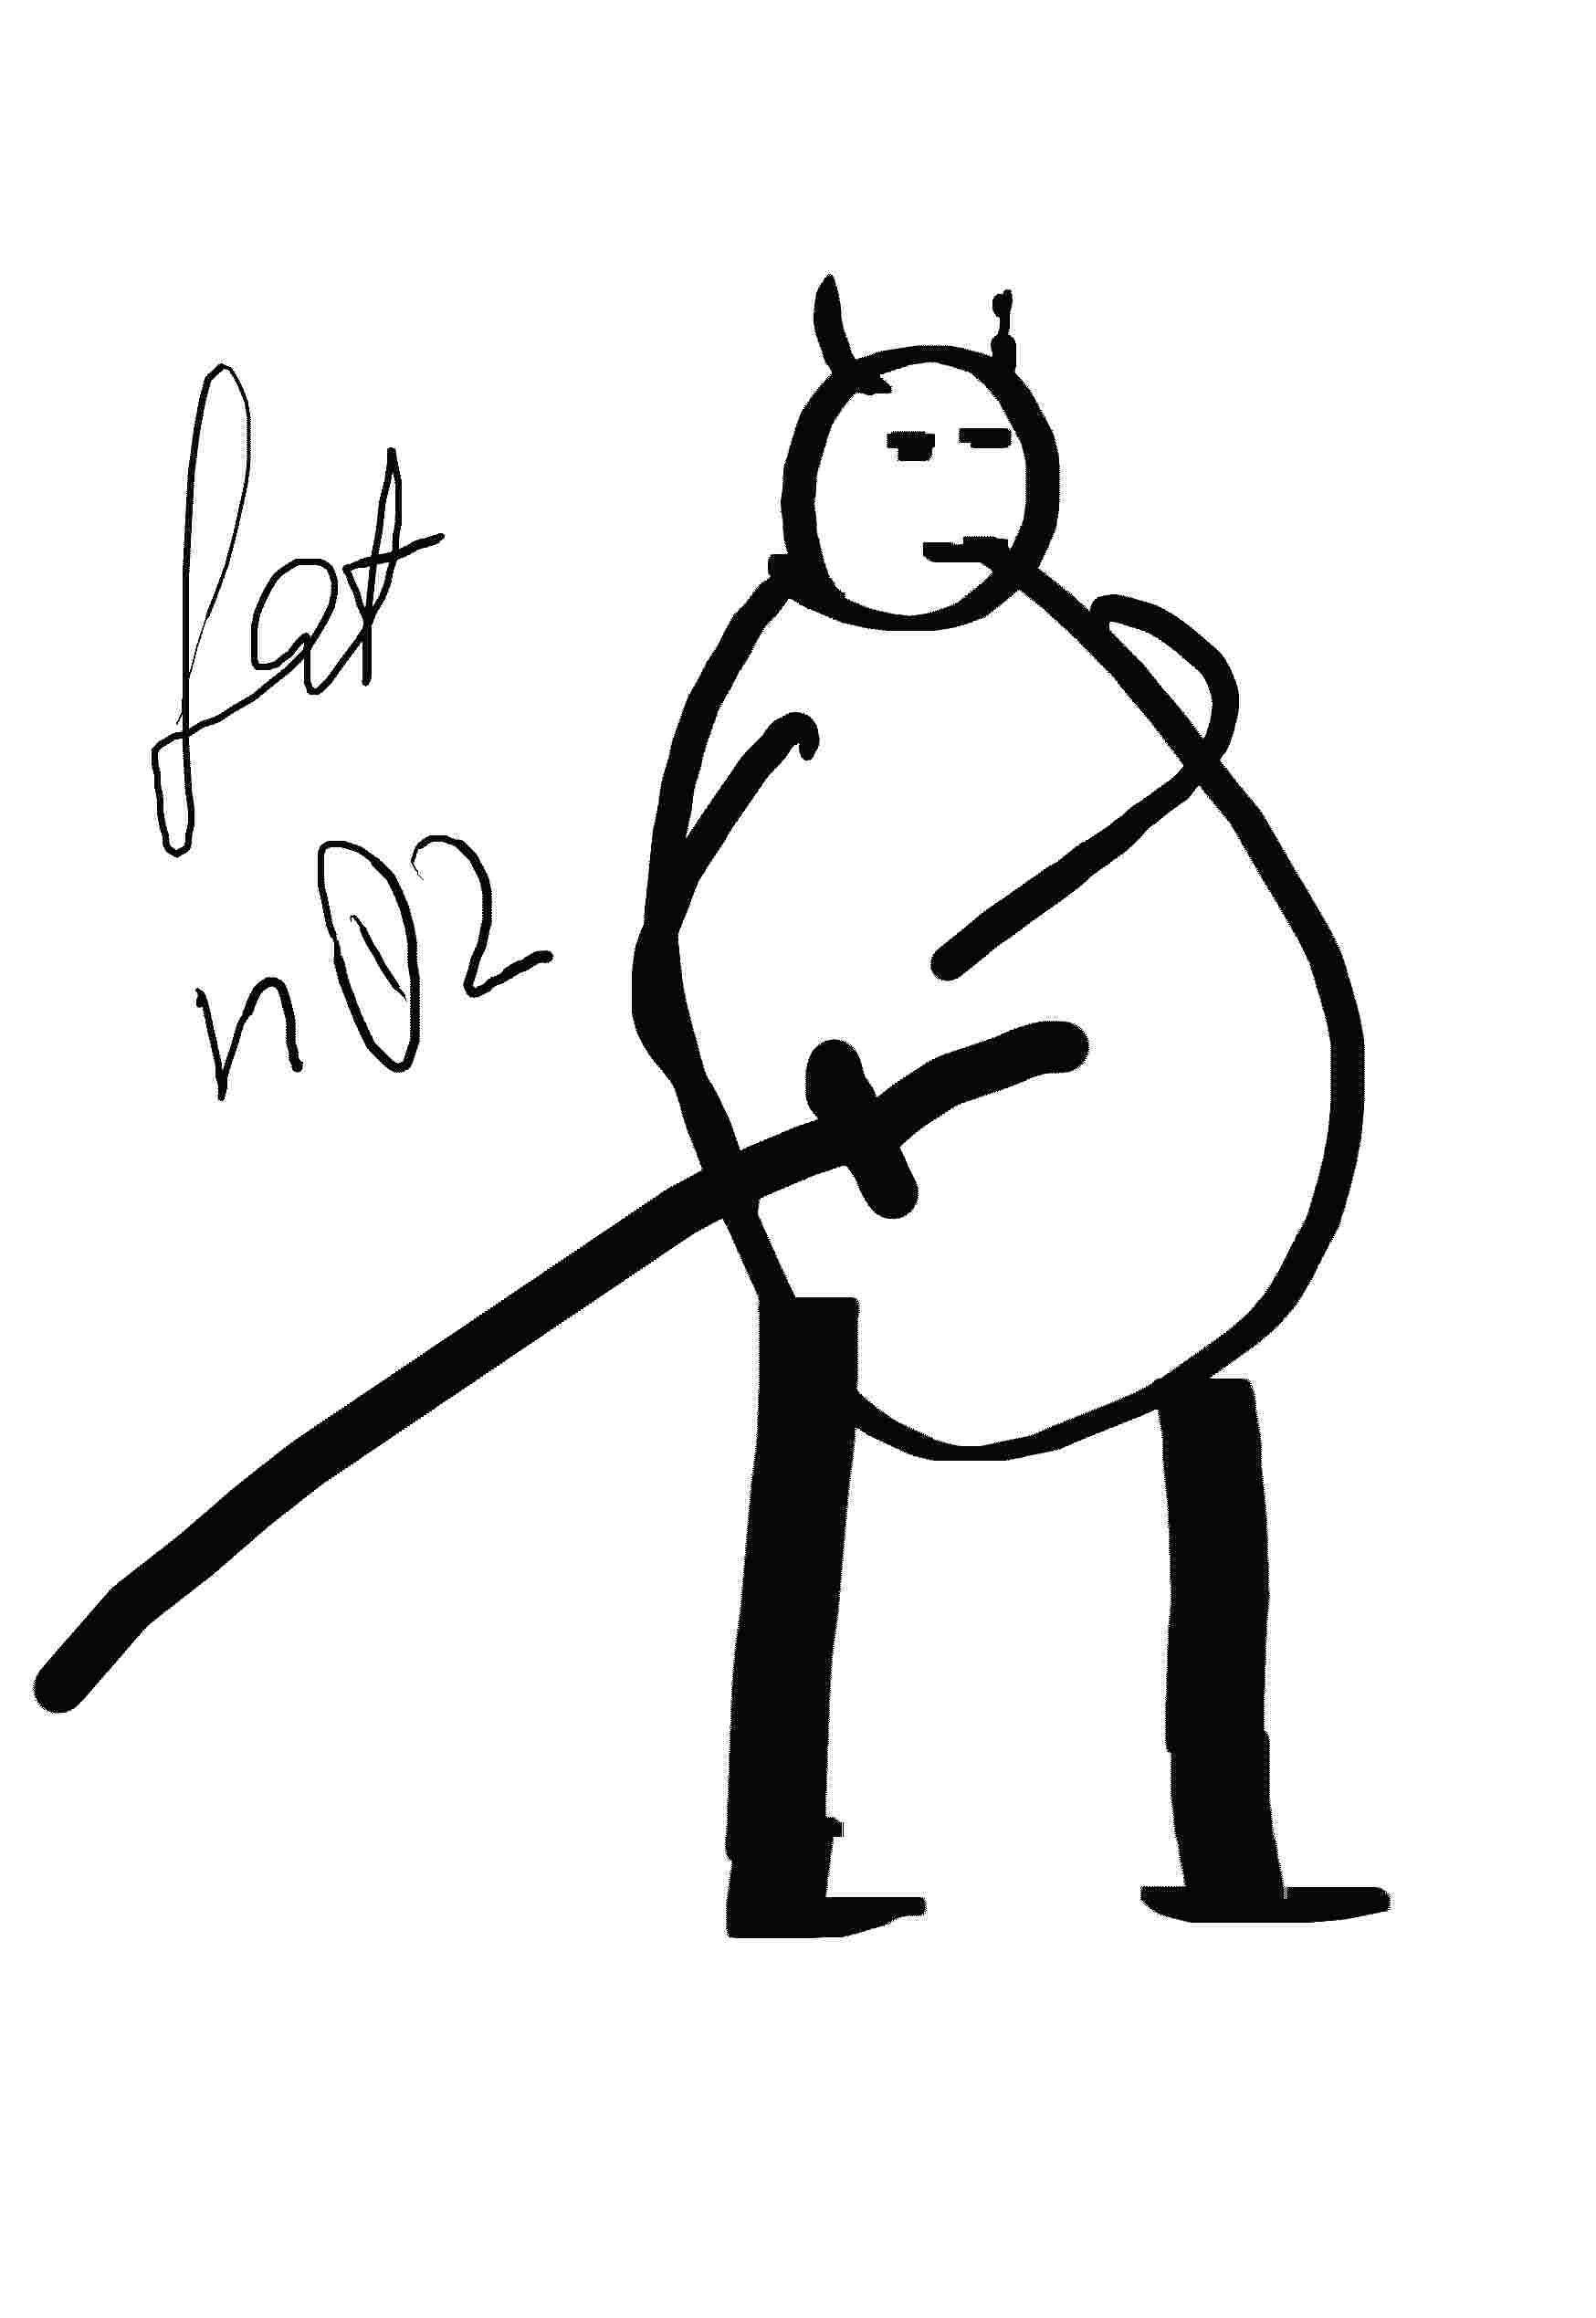
\includegraphics[width=1.00\textwidth]{logo.jpg}
\end{figure}

\clearpage
by 0746 \newline
An Open Kaillera project


This is not an SRS or anything formal, just a documentation of my thoughts.
 For me, it helps to write down things so I don't loose sight of what is
 important and what is not.

\twocolumn

\tableofcontents


\section{Intro}
Another prototype for the open kaillera client to explore some new concepts.


\section{Purpose}

This prototype intends to utilize/explore the the following concepts:

\begin{itemize}
	\item exploring automatic code generation for cores
	\item 3+ players p2p
	\item non-linear predictor for delay masking
	\item variable delay?
\end{itemize}

\section{Why its called fat}

Something like non-linear predictor for delay masking algorithm is rather
 complex in terms of algorithemic time and space complexity compared to the
 constant time in my previous approach. With the philosophy of
 optimization in development that I've carried so far for this project, as lame
 and counterproductive as it was, I'd have never even considered something like
 this to exist in this project. My previous self would have called this "fat,"
 hence the name fat n02.


\section{before anything else: developing some sort of framework}

As awful as my sense of professionalism is, I'd write to re-write the commpon
 dependent files completely to support the new ideas and stuff.

\section{first: exploring automatic code generation for cores}
The ammount of time I waste re-hacking stuff is extraordinary in ratio to
 other things I work on. Even when I make simple changes, I forget to add
 simple things and then if I'm lucky, someone reports a bug that I can
 trace to that broken thing. It's just not that, even when I want to test
 simple concepts, I end up re-coding a lot of stuff that are conceptually
 domain independent. Of course, the most obvious way to reduce them is to
 program in more systematic manner for abstraction and what not as opposed
 to trying to optimize things the lame way. But since we're not going to
 worry about that in this project, might as well try some things I learneded
 in school:
 
 
\begin{figure}[h]
	\centering
		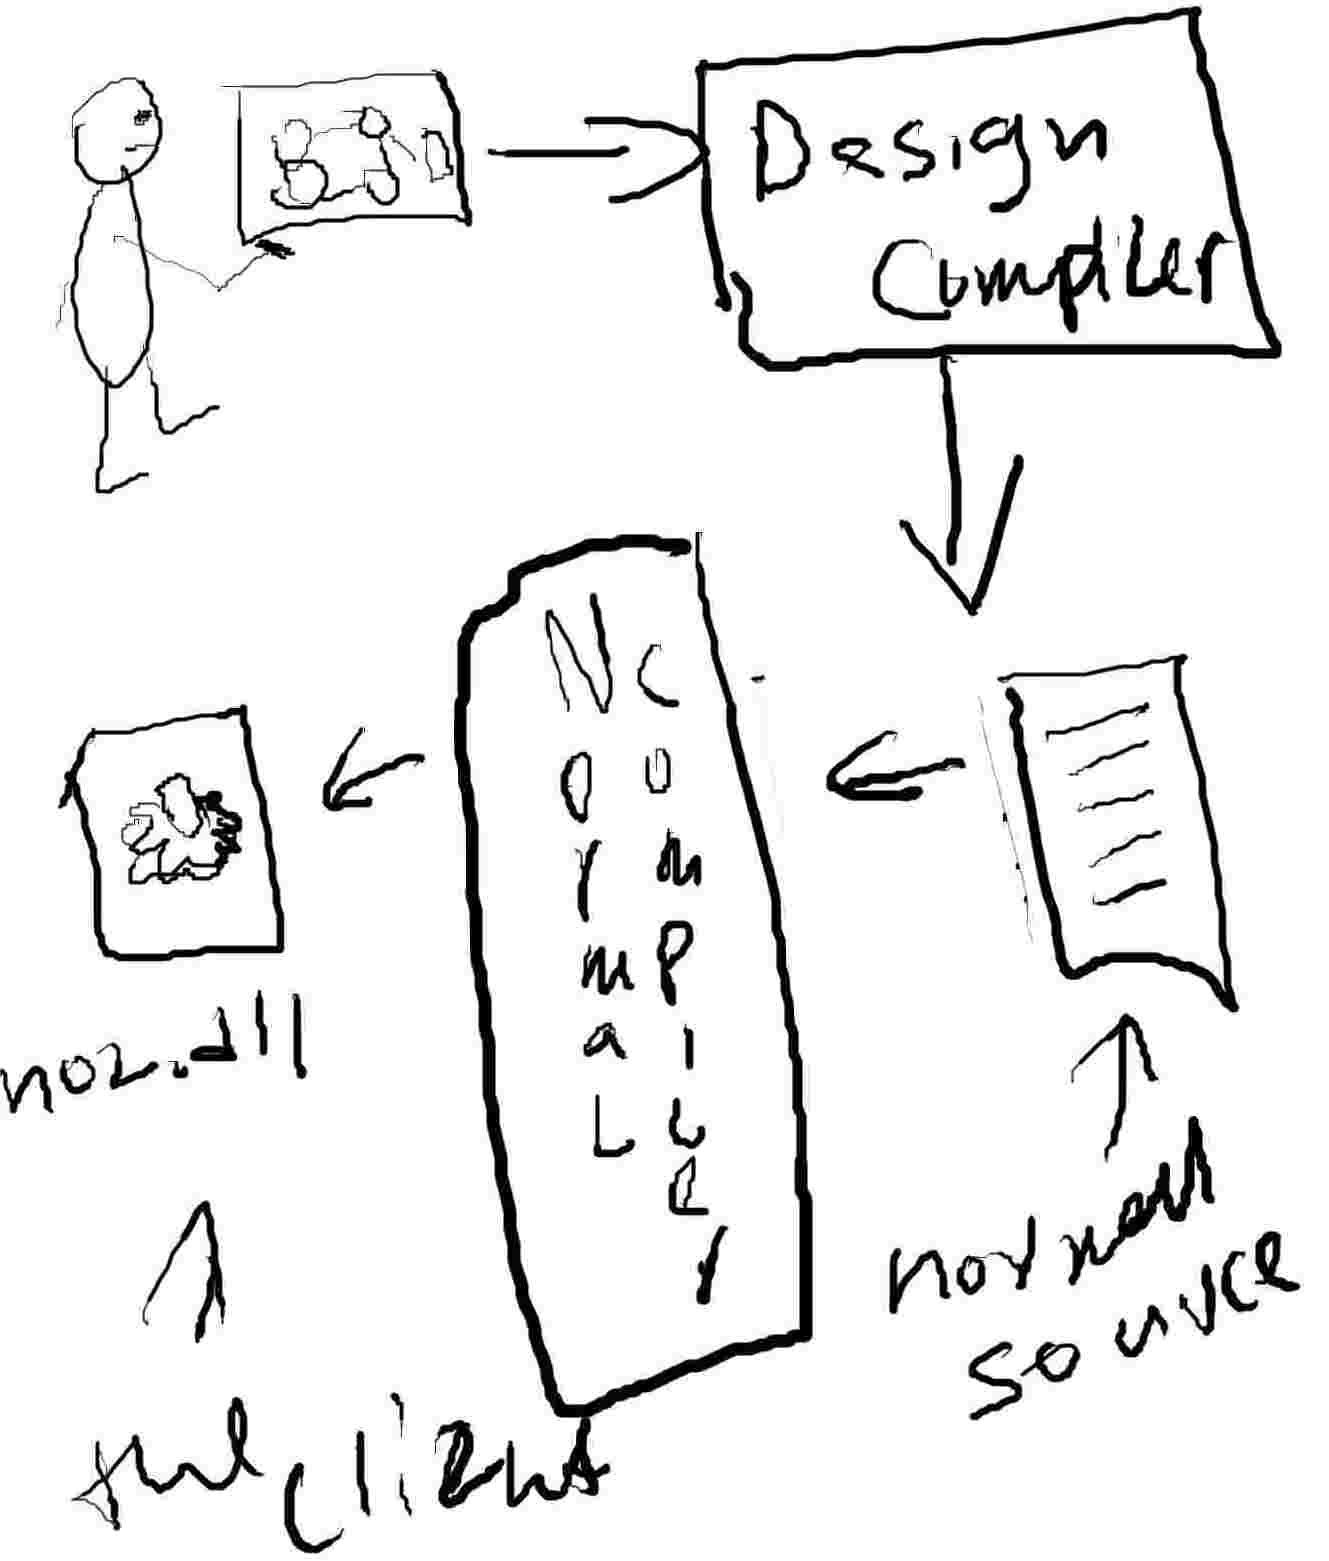
\includegraphics[width=0.50\textwidth]{idea1.jpg}
	\label{fig:idea1}
\end{figure}


\section{3+ players p2p}

\section{non-linear predictor for delay masking}

\section{variable delay?}




\end{document}
